% JAES condensed manuscript for paper 26325.
% Companion to the explanatory preprint sealed_driver_criteria.tex; shares
% figures, tables, and refs.bib, but sections_jaes/*.tex are independently
% written condensed prose (not \input-shared with the preprint).
\documentclass[fleqn]{jaes}

\jyear{2026}
%\jmonth{}
%\jvol{}
%\jnum{}

\usepackage{amsmath}\setlength{\mathindent}{10pt}
\usepackage{bm}
\usepackage{siunitx}
\usepackage{graphicx,booktabs,array}

\usepackage[capitalise]{cleveref}
  \crefformat{section}{\textsc{Sec.~#2#1#3}}
  \Crefformat{section}{\textsc{Sec.~#2#1#3}}
  \crefformat{figure}{{Fig.~#2#1#3}}
  \Crefformat{figure}{{Fig.~#2#1#3}}
  \crefformat{table}{{Table~#2#1#3}}
  \Crefformat{table}{{Table~#2#1#3}}

\numberwithin{equation}{section}

% refs.bib writes month fields as jan # {\slash} # feb, which BibTeX emits
% into the .bbl as "Jan.\slashFeb"; jaes.cls provides no such macro.
\providecommand{\slash}{/}
\providecommand{\slashFeb}{/Feb}
\hyphenation{elec-tro-acous-ti-cal loud-speak-er non-lin-ear-i-ties}

\newcommand{\Sd}{S_{\mathrm{d}}}
\newcommand{\Xmax}{X_{\mathrm{max}}}
\newcommand{\Vd}{V_{\mathrm{d}}}
\newcommand{\Mms}{M}
\renewcommand{\Re}{R_{\mathrm{e}}}
\newcommand{\Le}{L_{\mathrm{e}}}
\newcommand{\Rms}{R_{\mathrm{m}}}
\newcommand{\Cms}{C_{\mathrm{m}}}
\newcommand{\Bl}{Bl}
\newcommand{\Qes}{Q_{\mathrm{es}}}
\newcommand{\Qms}{Q_{\mathrm{ms}}}
\newcommand{\Qts}{Q_{\mathrm{ts}}}
\newcommand{\Qtc}{Q_{\mathrm{tc}}}
\newcommand{\Qmc}{Q_{\mathrm{mc}}}
\newcommand{\Vas}{V_{\mathrm{as}}}
\newcommand{\Vb}{V_{\mathrm{b}}}
\newcommand{\Pmax}{P_{\mathrm{max}}}
\newcommand{\ws}{\omega_{\mathrm{s}}}
\newcommand{\wc}{\omega_{\mathrm{c}}}
\newcommand{\se}{\sigma_{\mathrm{e}}}
\newcommand{\sm}{\sigma_{\mathrm{m}}}
\newcommand{\dd}{\mathrm{d}}

\begin{document}

% Title portion
\title{Datasheet-Based Ranking of Sealed-Box Bass Drivers for a Small-Area
DSP-Integrated Stereo System}

\markboth{HOLTKAMP}{DATASHEET-BASED RANKING OF SEALED-BOX BASS DRIVERS}

\authorgroup{
\author{LUC HOLTKAMP\thanks{To whom correspondence should be addressed, email: luc@sensemagic.nl.}}
\email{(luc@sensemagic.nl)}
\affil{SenseMagic, Netherlands}
}

\abstract{%
This Engineering Report gives a parameterized, reproducible pre-purchase
procedure for sealed-box bass-driver selection in a prepared couch or
mastering area. Classical relations are assembled into room-specific
displacement demand, displacement- and dissipation-limited ceilings, finite
voltage/current/power requirements, inductance and Doppler indicators, and
a numerical short-time excursion factor. A preferred alignment and
per-driver box cap replace hard $Q_{\mathrm{tc}}$ rejection: equalization
cost appears explicitly in excursion, electronics and burst response.
Candidates pass hard gates, enter role-specific Pareto fronts, and are
assembled into separate-radiator or stereo full-band systems compared on
six non-compensatory objectives. Crossover and 108-scenario architecture
sweeps test rather than assume role specialization. In the canonical
data-complete case the split architecture has feasible Pareto members
whereas the allowed full-band stereo search has none; permitting missing
inductance yields one unresolved survivor. Across the wider sweep,
full-band systems share fronts at lower targets but disappear at
\SI{115}{dB}. Aggregate evidence is reported
from a frozen private population, while a public Dayton/Faital pair supplies
the reproducible example. The result is conditional on the stated
population and inputs, not a universal motor bound; built systems still
require large-signal, manifold and room measurement.}
\maketitle

\begin{keywords}
loudspeaker driver selection, sealed enclosure, Pareto ranking, room gain,
stereo bass, nonlinear headroom
\end{keywords}

\section{Introduction}
\label{sec:intro}

The problem is deliberately narrow: given a room, one fixed listening
position, a target SPL, a driver database, and unlimited-complexity DSP
between amplifier and driver, select sealed bass driver(s) that reach the
target with least \emph{non-correctable} distortion (correctable made
precise below). All drivers radiate into half space from a common baffle;
every ceiling below is a \emph{single}-channel quantity.

Two facts drive the argument. (i)~\emph{Room gain}: below a room-set corner
$f_{\mathrm{pz}}$, pressure at the listening position tracks cone
displacement rather than acceleration, so a sealed system with $F_c\simeq
f_{\mathrm{pz}}$ tapers off below its corner for free. (ii)~\emph{Two
regimes, two jobs}: near $F_s$ a sealed driver is displacement-limited
($\Vd=\Sd\Xmax$); an octave or more above, it is dissipation-limited
($\eta_0\Pmax$). We prove (\cref{thm:bound}) no single motor maximizes both,
so the two roles want physically different drivers.

We review the $EBP$ heuristic (\cref{sec:prevwork}), derive the two
ceilings and their crossover (\cref{sec:freq,sec:time}), collect the
resulting invariants and the motor-materials bound (\cref{sec:invariants}),
show three independent non-correctable distortion mechanisms all reduce to
the same headroom ranking (\cref{sec:distortion}), close the low end with
the room (\cref{sec:roomclose}), and assemble an ordered, datasheet-only
selection procedure (\cref{sec:procedure}). \Cref{app:vented} proves, rather
than assumes, why the paper restricts itself to sealed enclosures, and
\cref{app:example} works a full numerical example.

\section{Previous work and positioning}
\label{sec:prevwork}

\Cref{tab:prior-art} lists, element by element, which parts of the
procedure are established prior results reused unchanged and which parts
are this report's own methodological or policy contribution. Nothing in
\cref{sec:model,sec:freq} is claimed as new physics.

\begin{table*}[htbp]
\centering
\caption{Established prior results integrated by this report vs. its own methodological and policy contribution.}
\label{tab:prior-art}
\begin{tabular}{p{5.1cm}p{2.6cm}p{6.7cm}}
\toprule
element & class & this report's treatment\\
\midrule
Sealed-box alignment, Thiele/Small closed-box theory & established prior result & reused unchanged as the sealed-box ODE and alignment line\\
Displacement-limited output ceiling ($V_d=S_dX_{\max}$) & established prior result & used as an exact descriptor, not a universal loudspeaker optimum\\
Thermal (dissipation-limited) output ceiling ($\eta_0P_{\max}$) & established prior result & used as an exact descriptor; never summed with the displacement ceiling\\
$X_{\max}$ as an IEC/Klippel excursion anchor & established prior result & used only as the clipping boundary; not converted into absolute THD\\
Room pressure-zone compliance below the first mode & established prior result & extended with an explicit first-order leakage-corner term; used only as a first-pass sizing/limiting model, not a claim about the complete room\\
Doppler (FM) sideband index & established prior result & reported as a separate, non-summed nonlinear-risk indicator\\
Finite-band DSP room correction & established prior result & adopted as an explicit scope input rather than an unconstrained assumption\\
Role-specific, non-compensatory ranking policy (mono sub manifold vs. independent stereo upper-bass channels) & this report's contribution & declared engineering policy; separate Pareto fronts per role, no cross-role or cross-channel summing credit\\
Explicit finite-amplifier feasibility gates (voltage, current, continuous and burst power) & this report's contribution & integrated into every role evaluation and the worked example\\
Numerical sealed-ODE transient (burst) displacement factor & this report's contribution & replaces a constant free-mass burst factor near $F_c$\\
Aggregate, hash-verified private-database screening evidence & this report's contribution & counts and hexbin/histogram population evidence only, no row-level redistribution\\
\bottomrule
\end{tabular}
\end{table*}


\textbf{Alignment and output ceilings.} Closed-box small-signal analysis
and synthesis \cite{small1972} and direct-radiator system analysis
\cite{small1972direct} supply the sealed-box model, the alignment relation,
the reference efficiency $\eta_0$, and the displacement- and
dissipation-limited output ceilings used throughout. Fielder and Benjamin
\cite{fielder1988} established the corresponding program-material and
room-aware view of subwoofer displacement requirements, which is the
closest prior work to the sizing part of the present procedure.

\textbf{Ratings and their comparability.} Continuous power ratings follow
different standards \cite{aes2}, and published $\Xmax$ values may be
geometric, distortion-defined, or vendor-specific
\cite{iec62458,klippel2003xmax,klippel2006}. Both introduce enough spread
between manufacturers to change a ranking, which is why the procedure
carries these as declared uncertainty inputs
(\cref{sec:scope}) and reports rank robustness against them
(\cref{sec:procedure}).

\textbf{$EBP$ as a screening heuristic.} $EBP\lesssim\SI{50}{\hertz}$
suggesting sealed and $\gtrsim\SI{100}{\hertz}$ suggesting vented
\cite{dickason2006} is a widely used enclosure-\emph{type} screen. It is a
motor-to-mass ratio and, through the exact corner rate $F_s/\Qts$, fixes
where a chosen $\Qtc$ places the box corner; it does not state achievable
output or nonlinear headroom. Here it enters only through the exact
$F_s/\Qts$ used in \cref{eq:alignment}, never as a standalone ranking key.
The approximation $F_s/\Qts\approx EBP$ is not used numerically: it differs
by $(1+\Qes/\Qms)$, which reaches several per cent to over ten per cent for
typical bass drivers.

\textbf{Why role specialization is worth testing.} A limited overhung-motor
scaling follows from the same standard identities. Let $u=h_c/h_g>1$ be
the winding-height/effective-gap-height ratio, let total conductor length
be $\ell$ and area $A_w$, and assume uniform gap flux $B$, conductor
conductivity $\sigma_c$, density $\rho_c$, and coil mass
$m_c=\rho_c\ell A_w$. With only the fraction $1/u$ of the winding in the
effective gap,
\begin{equation}
	\begin{gathered}
		\Bl\simeq\frac{B\ell}{u},\qquad
		\Re=\frac{\ell}{\sigma_cA_w},\qquad
		m_c=\rho_c\ell A_w,\\
		\boxed{\ \frac{F_s}{\Qes}u^2
		=\frac{B^2\sigma_c}{2\pi\rho_c}\frac{m_c}{\Mms}\ } .
	\end{gathered}
	\label{eq:motor-scaling}
\end{equation}
Thus, at fixed flux, material and coil-mass allocation, obtaining more
geometric overhang tends to trade against electrical damping per moving
mass. This is motivation to \emph{compare} a high-stroke low-bass role
with a lower-excursion upper-bass role. It is not a motor bound: $B$,
effective gap, $u$, coil-mass fraction, fringing and topology are normally
absent from datasheets, and expensive high-flux motors can move the
tradeoff. The relation is therefore never a feasibility gate or ranking
key. The architecture comparison of \cref{sec:procedure-architecture}
tests the practical consequence directly and retains any full-band
candidate that passes the same system gates.

\textbf{Large-signal behaviour and nonlinear risk.} Motor and suspension
nonlinearity, and the parameters used to characterize it, are surveyed by
Klippel \cite{klippel2006}; $\Xmax$ definitions and their measurement are
treated in \cite{klippel2003xmax}. Doppler (FM) distortion in
direct-radiator loudspeakers was described by Klipsch \cite{klipsch1969},
and its magnitude and audibility were subsequently disputed by Allison and
Villchur \cite{allison1982}; the present report therefore reports the
small-index first-sideband ratio and cites that debate rather than
converting it into a perceptual penalty. Thermal compression and power
handling follow Button \cite{button1992}. Perceptual thresholds for low-frequency
loudspeaker distortion depend on order, spectrum, level, and program
material \cite{fielder2019}, so no absolute audibility claim is made here.

\textbf{Ports.} Port compression, turbulence, and nonlinearity are
characterized in \cite{salvatti2002,vanderkooy1998}. These references
support the scoped discussion in \cref{app:vented}, which motivates the
choice of sealed loading for this application without claiming general
superiority.

\textbf{Room and correction.} The distinction between direct/early-field
and modal-region behaviour, and the interaction of loudspeakers with small
rooms, follows Toole \cite{toole2006}. Optimization over a defined seating
area using multiple subwoofers \cite{welti2006} is the explicit contrast to
the compact-area objective adopted here. Modal equalization
\cite{makivirta2003} and the review of room-response equalization
\cite{cecchi2018} bound what finite-band correction can achieve, and
motivate treating DSP correction as band-limited and regularized rather
than as exact inversion.

\textbf{Spatial attributes.} Scene-based spatial-quality terminology
\cite{rumsey2002} separates image and scene attributes from environmental
envelopment; small-room reflection effects are quantified in
\cite{bech1998}; envelopment's dependence on late lateral energy
\cite{bradley1995} and listener preference across reproduction methods
\cite{francombe2017} are the counterpoint that keeps
\cref{sec:intro-fidelity}'s claim restricted to scene fidelity.

What is missing from this body of work, and what this report supplies, is
not a new physical relation but a complete, reproducible, datasheet-only
decision path from a candidate population to a ranked, gate-checked
shortlist for one declared architecture, including the finite amplifier,
the finite enclosure, the room, and the transient case.

\section{Scope, conventions, and assumptions}
\label{sec:scope}

This section is the contract for everything that follows. SI units
throughout; $\rho_0=\SI{1.20}{\kilogram\per\cubic\meter}$,
$c=\SI{343}{\meter\per\second}$. Sound pressure levels are dB re
$p_0=\SI{20}{\micro\pascal}$ computed from \emph{rms} pressure, half-space
radiation, on axis.

\begin{center}
	\small
	\begin{tabular}{@{}llll@{}}
	\toprule
		$F_s$ & free-air resonance & $\Mms$ & moving mass\\
		$\Qes,\Qms,\Qts$ & Q factors & $\Re$ & DC resistance\\
		$\Vas$ & compliance vol. & $\Bl$ & force factor\\
		$\Sd$ & piston area & $\Le$ & coil inductance\\
		$\Xmax$ & linear excursion & $\Pmax$ & rated power\\
		$\Vd$ & displacement vol. & $\Vb$ & box volume\\
		$F_c,\Qtc$ & in-box corner, $Q$ & $f_L$ & inductive screen\\
	\bottomrule
	\end{tabular}
\end{center}

\subsection{Reference bases}
\label{sec:scope-bases}

Four distinct pressure references are used, and no figure or table mixes
them:

\begin{enumerate}
\item[B1.] \emph{Intrinsic ceiling}: one driver, half space,
	$r=\SI{1}{\meter}$. Used only to characterize a driver, never to assess
	a system.
\item[B2.] \emph{Couch-area reference demand}: the level required at the
	declared listening distance $r_{\mathrm{listen}}$ over the primary
	listening area. All feasibility checks use this basis.
\item[B3.] \emph{Mono manifold total}: the aggregate level of the complete
	low-bass manifold at B2. The per-driver share of the required displaced
	volume is the total divided by the number of manifold drivers.
\item[B4.] \emph{One independent stereo channel}: the level of one
	upper-bass channel at B2, with no credit from the opposite channel.
\end{enumerate}

Electrical quantities are per \emph{physical} driver, since each has its
own amplifier channel. Peak and rms conventions are stated at each
equation: displacements and the displaced volume $V_{\mathrm{dem}}$ are
peak values, while voltage, current, and power are rms over the evaluated
waveform.

\subsection{Canonical scenario}
\label{sec:scope-scenario}

The worked scenario used for every figure and table is:

\begin{center}
	\small
	\begin{tabular}{@{}p{2.5cm}p{5.0cm}@{}}
	\toprule
		room & $V_{\mathrm{room}}=\SI{60}{\cubic\meter}$,
			$L_{\max}=\SI{6}{\meter}$\\
		room model & leaky pressure zone,
			$f_\ell=\SI{10}{\hertz}$\\
		listening distance & $r_{\mathrm{listen}}=\SI{3}{\meter}$\\
		bands & sub $15$--$\SI{80}{\hertz}$;
			upper bass $80$--$\SI{250}{\hertz}$\\
		targets & \SI{110}{dB} manifold total (B3);\\
		 & \SI{105}{dB} per stereo channel (B4)\\
		amplifier, per driver & $\SI{90}{\volt}$ rms, $\SI{15}{\ampere}$ rms,\\
		 & \SI{500}{\watt} continuous, \SI{1}{\kilo\watt} burst\\
		alignment ceiling & $\Qtc\le0.55$\\
		enclosure limit & $\Vb\le\min(10\Vas,\ \SI{1.0}{\cubic\meter}/N)$
			per driver; \SI{1.0}{\cubic\meter} total per role\\
		excursion & $\Xmax$ hard limit;
			$0.80$ preferred margin\\
		Doppler screen & first-sideband ratio $\le0.02$\\
		transient & one-cycle rectangular burst, 8 phases\\
	\bottomrule
	\end{tabular}
\end{center}

Target levels are maximum-output design tests. The pressure-zone corner of
this room is $f_{\mathrm{pz}}=c/2L_{\max}\simeq\SI{28.6}{\hertz}$.

\subsection{Assumptions}
\label{sec:scope-assumptions}

\begin{enumerate}
\item[A1.] \emph{Lumped-parameter LTI small-signal model.} The screening
	domain ends at $|x|=\Xmax$; operation below that boundary does not by
	itself establish linear behavior. Cone breakup is a $ka\gtrsim1$
	phenomenon above the bands considered here, so the rigid-piston premise
	is the same one the published T/S parameters already presume.

\item[A2.] \emph{Coil inductance neglected in the transfer relations.}
	$f_L=\Re/(2\pi\Le)$ is retained as a screening frequency only. $\Le$ is
	itself frequency- and level-dependent, so $f_L$ is a rough indicator of
	where the model degrades, not a sharp validity boundary.

\item[A3.] \emph{Baffled rigid piston, far field, $ka\lesssim1$}
	($a=\sqrt{\Sd/\pi}$): the monopole approximation underlying every SPL
	relation below.

\item[A4.] \emph{Lossless sealed box}, adiabatic air spring. Box losses are
	a second-order correction that the ranking does not depend on.

\item[A5.] \emph{$\Pmax$ is a continuous coil-dissipation rating}
	$\langle i^2\rangle\Re$. Published ratings follow different standards
	\cite{aes2}, so comparisons are meaningful only within one standard, and
	a rating uncertainty of a few dB is propagated explicitly
	(\cref{sec:procedure}). Thermal compression \cite{button1992} raises
	$\Re$ during sustained drive and detunes $\Qtc$ and $F_c$; it is
	reported as a risk indicator, not modelled.

\item[A6.] \emph{Amplifier limits are explicit inputs.} Voltage, current,
	continuous power, and burst power per physical driver are hard gates
	(\cref{eq:ampgates}). The scenario is considered viable only if the
	driver, enclosure, and room constraints bind before those limits.

\item[A7.] \emph{$\Xmax$ is used only as the clipping boundary.} A
	distortion-defined value \cite{iec62458,klippel2003xmax} is preferred;
	geometric values must be converted or flagged. Excursion utilization
	$\xi_x=X_{\mathrm{dem}}/\Xmax$ is a risk proxy, not predicted THD.
	Public large-signal measurements supersede the proxy wherever they
	exist.

\item[A8.] \emph{Room effects are separated from free-field ceilings.} The
	ceilings of \cref{sec:freq} are free-field driver properties; room
	demand enters only through \cref{sec:room}.

\item[A9.] \emph{Summation is restricted to the mono manifold.} The
	manifold's drivers carry one common signal in a compact arrangement
	(spacing $\ll$ wavelength, consistent with A3), so their volume
	velocities are taken as coherent at the couch-area reference: each
	driver supplies $1/N$ of the required displaced volume. Independent
	stereo channels receive no summing credit. Total radiated power is
	\emph{not} inferred from on-axis pressure summation, mutual radiation
	impedance is not modelled, and the electrical demand of each physical
	driver is computed from its own displacement across the complete role
	band.

\item[A10.] \emph{Nonlinear indicators are proxies.} They are
	leading-order, dimensionless screening quantities reported separately.
	They are not summed, and they are not converted into an absolute
	distortion percentage.

\item[A11.] \emph{DSP correction is finite-band and regularized.} Linear
	correction trades response error against displacement, voltage, current,
	thermal load, noise, and model error; it does not reduce nonlinear
	residuals, and its practical limits over an area are those reported in
	\cite{makivirta2003,cecchi2018}.
\end{enumerate}

\subsection{Limitations of public data}
\label{sec:scope-datalimits}

Datasheet fields carry mixed conventions for $\Xmax$, $\Pmax$, and $\Le$,
occasional missing fields, and no statement of unit-to-unit spread. The
procedure therefore (i) rejects records missing a required field rather
than imputing it, (ii) records which fields were derived rather than
published, and (iii) reports rank stability under declared perturbations of
$\Xmax$ and $\Pmax$ instead of presenting a single ranking as exact.

\section{Model and transfer relations}
\label{sec:model}

The relations in this section are classical
\cite{small1972,small1972direct} and are restated only to fix notation and
the peak/rms conventions used by the gates.

With terminal voltage $e(t)$, current $i(t)$, cone displacement $x(t)$,
electrical side $e=\Re i+\Bl\dot x$ (A2), force $F=\Bl i$, and total
stiffness $k_t=1/\Cms+\rho_0c^2\Sd^2/\Vb=(1+\alpha)/\Cms$ with
$\alpha\equiv\Vas/\Vb$:

\begin{equation}
	\boxed{\
		\ddot{x}+\sigma\dot{x}+\wc^2 x = \frac{\Bl}{\Re \Mms}\,e(t)\ }
	\label{eq:ode}
\end{equation}

where $\sigma\equiv\sm+\se$, $\sm\equiv\Rms/\Mms$,
$\se\equiv\Bl^2/(\Re\Mms)$, and $\wc^2\equiv k_t/\Mms$. Free air:
$\ws=2\pi F_s=\sqrt{1/(\Mms\Cms)}$, $\Qes=\ws/\se$, $\Qms=\ws/\sm$,
$\Qts=\ws/\sigma$. In box: $\wc=\ws\sqrt{1+\alpha}$, $\Qtc=\wc/\sigma$.

\subsection{Alignment line}
\label{sec:model-alignment}

Because $\sigma$ contains no stiffness term, it is enclosure-independent,
which gives the sealed alignment relation \cite{small1972}

\begin{equation}
	\boxed{\
		\frac{\wc}{\Qtc} = \frac{\ws}{\Qts} = \sigma
			\quad\Longleftrightarrow\quad
		F_c = \Qtc\,\frac{F_s}{\Qts}\ }
	\label{eq:alignment}
\end{equation}

with $\Vb=\Vas/((\Qtc/\Qts)^2-1)$ and $\Qtc>\Qts$. A sealed driver
therefore has exactly one free alignment parameter, its position along the
line $\wc=\Qtc\sigma$, and the \emph{corner rate}

\begin{equation}
	\frac{\sigma}{2\pi}=\frac{F_s}{\Qts}
		=EBP\left(1+\frac{\Qes}{\Qms}\right)
	\label{eq:cornerrate}
\end{equation}

is the datasheet quantity that decides where the corner can be placed for a
chosen $\Qtc$. The exact expression, not the $EBP$ approximation, is used
in every gate. The envelope decay rate of every sealed alignment of a given
driver is $\sigma/2=\pi F_s/\Qts$, so the enclosure selects only the damped
frequency and the overshoot pattern, not the decay rate.

\subsection{Steady-sine relations}
\label{sec:model-steady}

For steady sine excitation with peak displacement $\hat x$, peak current
$\hat\imath$, and peak terminal voltage $\hat e$ (rms values are
$1/\sqrt2$ of these):

\begin{align}
	\hat{x}(\omega)&=
		\frac{\Bl}{\Re\Mms}\,
		\frac{\hat{e}}{\sqrt{(\wc^2-\omega^2)^2+\sigma^2\omega^2}},
		\label{eq:xofe}\\
	\hat{\imath}(\omega)&=
		\frac{\Mms}{\Bl}\,
		\hat{x}\,\sqrt{(\wc^2-\omega^2)^2+\sm^2\omega^2},
		\label{eq:iofx}\\
	\hat{p}(\omega)&=
		\frac{\rho_0\Sd\,\omega^2\hat{x}}{2\pi r}\qquad\text{(A3)} .
		\label{eq:pofx}
\end{align}

Only mechanical damping $\sm$ appears in \cref{eq:iofx}: electrical damping
is a consequence of the current, not an additional load on it. The rms
pressure that enters every SPL below is $\hat p/\sqrt2$.

\section{Steady-state output ceilings and finite electrical demand}
\label{sec:freq}

Two driver limits bound steady sinusoidal output: linear excursion and
continuous coil dissipation. Both are established results
\cite{small1972direct}; they are restated here on the reference bases of
\cref{sec:scope-bases} so that the gates below are unambiguous.

\subsection{Displacement- and dissipation-limited ceilings}
\label{sec:freq-ceilings}

With $\Vd\equiv\Sd\Xmax$ (peak displaced volume) and
$\hat p_{\mathrm L}(\omega)=\rho_0\omega^2\Vd/(2\pi r)$, the
excursion-limited intrinsic ceiling (basis B1) is

\begin{equation}
	\boxed{\ \mathrm{SPL}_{\mathrm{L}}(f)=
			108.5+20\log_{10}\!\big(f^2\,\Vd\big)\ \mathrm{dB}\ }
	\label{eq:SPLL}
\end{equation}

(rms pressure, $r=\SI{1}{\meter}$, half space, $+12$\,dB/oct). It depends
on no other parameter: within this model $\Qtc$, $F_c$, $\Bl$, $\Re$,
$\Mms$, and $\Pmax$ do not appear, so in the excursion-limited regime
$\Vd$ alone orders candidates. The alignment governs corner placement,
settling, and the drive required to reach the ceiling, not the ceiling
itself.

With the reference efficiency

\begin{equation}
	\eta_0 =
		\frac{\rho_0}{2\pi c} \,
		\frac{\Bl^2\Sd^2}{\Re\Mms^2}
		= 9.78\times10^{-7}\ \frac{F_s^3\,\Vas[\mathrm{m^3}]}{\Qes},
	\label{eq:eta0}
\end{equation}

the dissipation-limited passband ceiling is

\begin{equation}
	\boxed{\ \mathrm{SPL}_{\mathrm{T}}=112.2+10\log_{10}\!\big(\eta_0\Pmax\big)\ \mathrm{dB}\ }
	\label{eq:SPLT}
\end{equation}

on the same basis, obtained by substituting $\hat\imath=\sqrt{2P/\Re}$ into
\cref{eq:iofx,eq:pofx}. The two ceilings combine as

\begin{equation}
	p_{\max}(\omega) =
		\frac{\rho_0\Sd\,\omega^2}{2\pi r}\;
		\min\!\Big\{\Xmax,\ X_{\mathrm{T}}(\omega)\Big\},
	\label{eq:master}
\end{equation}

and cross at

\begin{equation}
	f_x =
		\frac{1}{2\pi}\left(\frac{4\pi c\,\eta_0\Pmax}{\rho_0\,\Vd^{2}}\right)^{1/4} .
	\label{eq:fx}
\end{equation}

Below $f_x$ additional $\Vd$ raises the ceiling; above it additional
$\eta_0\Pmax$ does. These are \emph{ceilings}: adequacy is decided at the
target level of \cref{sec:room}, not at the ceiling, so a driver whose
regime boundary lies inside its band may still be far from either limit at
the declared target.

\subsection{Demand and finite amplifier gates}
\label{sec:freq-gates}

Let $V_{\mathrm{dem}}(f)$ be the peak displaced volume required at the
couch-area reference (basis B2--B4, \cref{sec:room}), and let the role be
served by $N$ identical drivers sharing one common signal (A9), so the
per-driver peak displacement is
$X_{\mathrm{dem}}(f)=V_{\mathrm{dem}}(f)/(N\Sd)$. Inverting
\cref{eq:xofe,eq:iofx} gives the exact steady requirements per physical
driver, in rms:

\begin{align}
	E_{\mathrm{req}}(\omega)&=
		\frac{\Re\Mms}{\sqrt2\,\Bl}\,X_{\mathrm{dem}}
		\sqrt{(\wc^2-\omega^2)^2+\sigma^2\omega^2},
		\label{eq:Ereq}\\
	I_{\mathrm{req}}(\omega)&=
		\frac{\Mms}{\sqrt2\,\Bl}\,X_{\mathrm{dem}}
		\sqrt{(\wc^2-\omega^2)^2+\sm^2\omega^2},
		\label{eq:Ireq}\\
	P_{\mathrm{req}}(\omega)&=
		\frac{\Mms\Qes X_{\mathrm{dem}}^{2}}{4\pi F_s}
		\Big[(\wc^2-\omega^2)^2+\sm^2\omega^2\Big] .
		\label{eq:Preq}
\end{align}

\Cref{eq:Preq} is a ``bathtub'' in $\omega$: minimum near $\wc$, finite at
DC, and rising both below the corner (the correction cost of holding a flat
target through the sealed roll-off, $12$\,dB/oct in power) and above it
(the $\omega^4$ growth of the pressure required from a fixed displacement).
Both branches must be evaluated across the complete role band, since the
worst voltage, worst current, and worst power generally occur at different
frequencies.

The feasibility gates are then, for every $f$ in the role band and for
every physical driver,
\begin{equation}
	\boxed{\
	\begin{aligned}
	E_{\mathrm{req}}&\le E_{\mathrm{amp}}, &
	I_{\mathrm{req}}&\le I_{\mathrm{amp}},\\
	E_{\mathrm{burst}}&\le E_{\mathrm{amp}}, &
	I_{\mathrm{burst}}&\le I_{\mathrm{amp}},\\
	P_{\mathrm{req}}&\le\min\{\Pmax,\ P_{\mathrm{amp,cont}}\}, &
	P_{\mathrm{burst}}&\le P_{\mathrm{amp,burst}},
	\end{aligned}\ }
	\label{eq:ampgates}
\end{equation}

with the burst quantities from \cref{sec:time}, together with
$\xi_x=X_{\mathrm{dem}}/\Xmax\le1$ (A7). A candidate failing any gate at
any frequency in its band is rejected, with the binding gate and frequency
recorded.

DSP correction is not free. Flattening the response below the corner
multiplies \cref{eq:Preq} by roughly $(\wc/\omega)^4$ and the required
displacement by $(\wc/\omega)^2$; it also raises current, coil temperature,
and---through the resulting rise in $\Re$ \cite{button1992}---detunes
$\Qtc$ and $F_c$ during sustained programme. Correction is therefore
applied over a finite band, and its cost is charged to
\cref{eq:Ereq,eq:Ireq,eq:Preq} rather than assumed away.
\Cref{fig:output-electrical} shows both sides of this check for both roles:
the margin of the combined ceiling \cref{eq:master} over the couch-area
target, and the resulting electrical demand against the declared limits.

\begin{figure}[htbp]
	\centering
	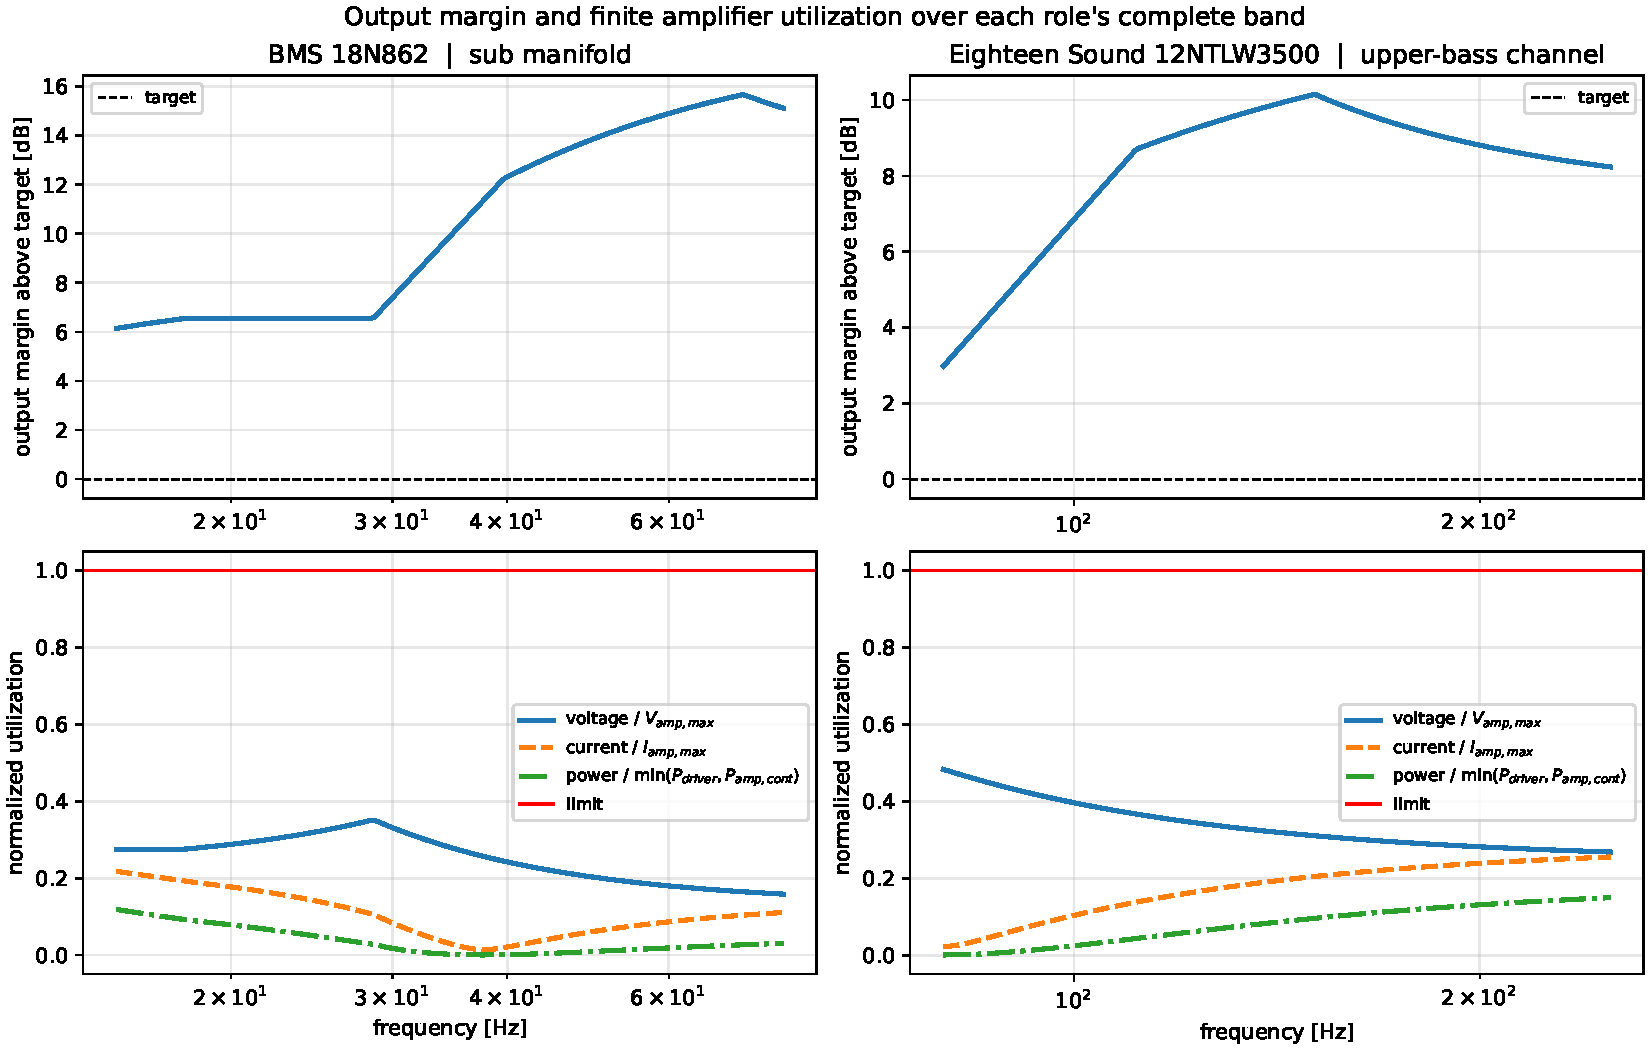
\includegraphics[width=\columnwidth]{../figures/fig_output_electrical}
	\caption{Output margin and finite amplifier utilization over each role's
	complete band, on one couch-area reference basis. Top: margin of the
	combined ceiling \cref{eq:master} above the role's target. Bottom:
	required rms voltage, current, and coil power per physical driver,
	\cref{eq:Ereq,eq:Ireq,eq:Preq}, normalized by the declared per-driver
	amplifier and driver limits. Left column: mono low-bass manifold; right
	column: one independent stereo upper-bass channel.}
	\label{fig:output-electrical}
\end{figure}

\section{Time domain: attack, overshoot, settling; the driver invariants}
\label{sec:time}

Model a bass attack as a one-cycle acceleration burst, $\omega\gg\wc$
(free-mass limit).

\begin{lemma}[Burst shape factor]
\label{lem:shape}
With $C\equiv \omega^2\max_t|x(t)|/A$: $C=1$ for steady sine; for one-cycle
sine-phase bursts $C=2\pi$, cosine-phase $C=2$; $n$ cycles, sine phase,
$C=2\pi n$. Transient program thus demands $C\in[2,2\pi]$
($6$--$16$\,dB) more excursion per unit peak pressure than steady sine.
\end{lemma}

Peak-equivalent ceilings become
\begin{align}
\hat L_{\mathrm{L,burst}}(f)&=108.5+20\log_{10}(f^2\Vd)-20\log_{10}C,
\label{eq:burstL}\\
\hat L_{\mathrm{T,burst}}&=112.2+10\log_{10}(\eta_0\,\kappa\Pmax),
\label{eq:burstT}
\end{align}
with $\kappa$ (A5) the short-term dissipation headroom.

\begin{proposition}[Equivalence of the two analyses; boundary shift]
\label{prop:equiv}
Time- and frequency-domain limits yield the same two figures of merit,
$\Vd$ and $\eta_0\Pmax$, rescaled by $C$ and $\kappa$. The regime boundary
moves up to
\begin{equation}
\hat f_x=f_x\,(\kappa C^2)^{1/4}
\qquad(\kappa=4,\ C=2\ \Rightarrow\ \hat f_x=2f_x).
\label{eq:fxburst}
\end{equation}
\end{proposition}

So for attack-type program the excursion regime extends roughly an octave
higher than the sine analysis suggests; both roles need both FOMs checked at
their own band edge.

\begin{proposition}[Settling is a driver constant; ring shape is a box choice]
\label{prop:decay}
The envelope decay rate of every sealed alignment of a given driver equals
$\sigma/2=\pi F_s/\Qts$ (box-invariant, \cref{prop:invariance}); the box
selects only $\omega_d$ and the overshoot pattern. Step-response overshoot
$M_p=\exp(-\pi\zeta/\sqrt{1-\zeta^2})$, $\zeta=1/(2\Qtc)$: $M_p\le1\%
\Leftrightarrow\Qtc\le0.61$; $M_p\le5\%\Leftrightarrow\Qtc\le0.72$.
\end{proposition}

Spurious ring-down tail pressure satisfies
$\hat p_{\mathrm{tail}}/\hat p_{\mathrm{burst}}\le C(\wc/\omega)^{2}$
(worst phase), improving 12\,dB/oct with corner-below-band separation --- an
LTI, hence FIR-correctable, effect (at the cost of \eqref{eq:EQtax}). The
invariants FIR cannot touch remain $\Vd$, $\eta_0\Pmax$, $\sigma$.

\subsection{The driver invariants, and what \texorpdfstring{$EBP$}{EBP} actually is}
\label{sec:invariants}

Four quantities survive both analyses unchanged: $\Vd=\Sd\Xmax$ (excursion
regime); $\eta_0\Pmax$ (dissipation regime, \eqref{eq:eta0}); the corner
rate $\sigma/2\pi=F_s/\Qts$ (placement, settling); and $f_L=\Re/(2\pi\Le)$
(upper validity). Cone area $\Sd$ enters again separately, via Doppler
(\cref{sec:distortion}).

A common rule of thumb states $EBP\propto V_c/\Mms$ as a motor-strength
proxy; here is the exact version. For an overhung motor with coil conductor
mass $m_c$, conductivity $\sigma_c$, density $\rho_c$, flux density $B$, and
effective overhang factor $u\ge1$:
\begin{equation}
\se=\frac{\Bl^2}{\Re\Mms}=\frac{B^2\sigma_c}{\rho_c}\cdot\frac{m_c}{\Mms}\cdot\frac{1}{u^2}.
\label{eq:sebound}
\end{equation}

\begin{theorem}[Motor materials bound]
\label{thm:bound}
For an overhung motor, equality holds in \eqref{eq:sebound}:
$EBP\cdot u^{2}=K_{\mathrm{mat}}\cdot\dfrac{m_c}{\Mms}$, with
$K_{\mathrm{mat}}\equiv\dfrac{B^{2}\sigma_c}{2\pi\rho_c}$ (copper:
$1059\,B^2$\,Hz; aluminium: $2063\,B^2$\,Hz). Bounding the coil-mass
fraction, $m_c/\Mms\le\beta_{\max}\lesssim0.35$, gives
\begin{equation}
\boxed{\ EBP\cdot u^{2}\;\le\;K_{\mathrm{mat}}\,\beta_{\max}\ }
\label{eq:thmbound}
\end{equation}
\end{theorem}

At $B=1.0$--$1.2$\,T (Cu, $\beta_{\max}=0.35$) the bound is
$\approx370$--$530$\,Hz: a sub-class driver ($u\approx3$) is limited to
$EBP\lesssim45$\,Hz, an attack-class corner rate of $135$\,Hz forces
$u\lesssim1.8$. A single driver combining sub-class stroke and attack-class
corner rate would need $\beta B^2\approx1.1$ --- impossible. Three
independent mechanisms enforce the split: \eqref{eq:thmbound} itself
(stroke suppresses corner rate quadratically); \cref{prop:invariance} (one
driver has one $\sigma$, hence one $F_c$); and A2 (tall coil $\Rightarrow$
large $\Le$ $\Rightarrow$ low $f_L$ intruding into the attack band).
Escape routes (underhung/XBL$^2$, dual gap, shorting rings, aluminium
coils) buy factors of $\sim2$, not the required $\sim5$, trading against
$\beta$ or $B$ inside the same bound.

$\beta_{\max}$ is an observed ceiling on real motor construction (coil
formers, adhesives, winding density), not a law of electromagnetism, and
neither $m_c$ nor $B$ is a standalone datasheet field. Since $u\ge1$,
however, \eqref{eq:thmbound}'s equality also gives a lower bound
computable from $EBP$ alone: $m_c/\Mms\ge EBP/K_{\mathrm{mat}}(B)$,
independent of the otherwise-unmeasurable $u$. \Cref{tab:ebp-census}
applies this to $N=1025$ bass-relevant drivers (VituixCAD database, Type
S/W/WM): at a conservative $B=1.0$\,T (copper), only $0.3\%$ approach
$\beta_{\max}$, and the material-agnostic (aluminium) bound is never
exceeded; the single outlier needs only $B\approx1.4$\,T (a plausible
neodymium motor) to reach the ceiling, not exceed it.

\begin{table*}[htbp]
\centering
\caption{Lower-bound coil-mass fraction $\beta_{\min}=EBP/K_{\mathrm{mat}}(B)$ (Thm.~\ref{thm:bound} at $u{=}1$, Cu $B{=}1.0$\,T unless noted) over $N{=}1025$ bass-relevant drivers (Type S/W/WM) in the bundled VituixCAD database, vs.\ $\beta_{\max}\approx0.35$.}
\label{tab:ebp-census}
\small
\begin{tabular}{lc}
\toprule
quantity & value\\
\midrule
$N$ & 1025\\
median $\beta_{\min}$ & 0.10\\
$p_{90}/p_{99}/p_{99.5}$ & 0.17 / 0.29 / 0.31\\
max & 0.66 (B\&C Speakers 8NSM64, needs $B{\approx}1.37$\,T)\\
material-agnostic (Al) excess & 0.0\%\\
\bottomrule
\end{tabular}
\end{table*}


\section{Nonlinear-risk indicators and ranking policy}
\label{sec:risk}

The ceilings of \cref{sec:freq} rank candidates by output capability. What
remains is the risk that a candidate, while formally inside its gates,
operates closer to its nonlinear regions than an alternative. Linear
correction does not help here: a linear pre-filter cannot reduce a
nonlinear residual for all programme material, because if it did, scaling
the input would force that residual to be linear.

This report does \emph{not} convert $\Xmax$, or any of the indicators
below, into an absolute distortion figure, and does not add unlike
indicators into a scalar total. They occur at different frequencies, with
different phases and different perceptual weights
\cite{klippel2006,allison1982,fielder2019}, so a sum would not correspond
to any measurable quantity. They are reported as a vector of separately
named, dimensionless indicators.

\subsection{Reported indicators}
\label{sec:risk-vector}

For each role evaluation the procedure reports

\begin{equation}
	\mathbf r=\big(\xi_x,\ \xi_x^{\mathrm{tr}},\ d_{\mathrm D},\
		\xi_{\mathrm{box}},\ \xi_P,\ \xi_{\mathrm{amp}},\
		f_{\mathcal B,\mathrm h}/f_L,\ V_{\mathrm b}^{\mathrm{tot}}\big) .
	\label{eq:riskvec}
\end{equation}

\textbf{Excursion utilization} $\xi_x=X_{\mathrm{dem}}/\Xmax$ and its
transient counterpart $\xi_x^{\mathrm{tr}}$ \cref{eq:xitr}. Expanding motor
force factor and suspension compliance about the rest position gives
even- and odd-order terms that grow with $\xi_x$, which is the motivation
for using utilization as a screening indicator; the coefficients are not
available from datasheets, so no distortion percentage is inferred.
$\xi_x=1$ is the hard clipping boundary (A7). The value $0.80$ is a
\emph{preferred} design margin---about $\SI{1.9}{dB}$ of excursion
headroom---used as a lexicographic preference and to size unit counts, not
as a rejection threshold and not as a distortion budget.

\textbf{Doppler sideband indicator.} For a role band $\mathcal B$, define
$X_{\mathcal B}=\max_{f\in\mathcal B}X_{\mathrm{dem}}(f)$ and let
$f_{\mathcal B,\mathrm h}$ be its upper edge. A component at
$f_{\mathcal B,\mathrm h}$ radiated from a cone moving with peak
$X_{\mathcal B}$ acquires the phase-modulation index
$m=2\pi f_{\mathcal B,\mathrm h}X_{\mathcal B}/c$. For small $m$, either
first-order sideband has amplitude ratio $J_1(m)/J_0(m)\simeq m/2$, so the
reported indicator is

\begin{equation}
	d_{\mathrm D}\equiv\frac{J_1(m)}{J_0(m)}
	\simeq\frac{\pi f_{\mathcal B,\mathrm h}X_{\mathcal B}}{c},
	\qquad
	X_{\mathcal B}=\max_{f\in\mathcal B}
		\frac{V_{\mathrm{dem}}(f)}{N\Sd} .
	\label{eq:doppler}
\end{equation}

The phase modulation is kinematic and exact within the rigid-piston model;
the sideband approximation is its small-index limit. At fixed output,
$d_{\mathrm D}$ falls as $1/\Sd$: among candidates with equal $\Vd$, the
larger cone has the lower indicator. It is \emph{not} a perceived
distortion value---the audibility of loudspeaker FM distortion has been
disputed since \cite{klipsch1969,allison1982}---and is used only as a
screen against a declared sideband-ratio budget. Splitting the bands
removes cross-band modulation \emph{on the same radiator}; it does not
remove self-modulation within a band, and finite crossover overlap leaves
some residual.

\textbf{Box-spring indicator.} Adiabatic compression of the enclosed air is
an asymmetric spring; weighting the leading term by the box's share of
total stiffness gives

\begin{equation}
	\xi_{\mathrm{box}} \approx
		\frac{\gamma+1}{4}\,
		\frac{V_{\mathrm{dem}}}{N\Vb}\Big(1-\frac{\Qts^2}{\Qtc^2}\Big),
	\label{eq:boxHD}
\end{equation}

a property of the enclosure rather than the motor, reduced by larger
$\Vb$ and by stuffing ($\gamma_{\mathrm{eff}}\to1$). It is reported
separately and never added to \cref{eq:doppler} or to $\xi_x$.

\textbf{Electrical and thermal utilization.} Let
\begin{equation}
	\begin{aligned}
	\xi_P &={P_{\mathrm{req}}}/{\Pmax},\\
	\xi_{\mathrm{amp}}&=\max\!\left\{
		\frac{\max(E_{\mathrm{req}},E_{\mathrm{burst}})}
		     {E_{\mathrm{amp}}},
		\frac{\max(I_{\mathrm{req}},I_{\mathrm{burst}})}
		     {I_{\mathrm{amp}}},\right.\\[-0.3ex]
	&\hspace{4.5em}\left.
		\frac{P_{\mathrm{req}}}{P_{\mathrm{amp,cont}}},
		\frac{P_{\mathrm{burst}}}{P_{\mathrm{amp,burst}}}
		\right\}.
	\end{aligned}
\end{equation}
These follow from \cref{eq:ampgates}. $\xi_P$ is a warning indicator only:
inferring coil temperature would require thermal resistances and time
constants that datasheets do not publish \cite{button1992}, and $\Pmax$
itself carries standard-dependent uncertainty (A5).

\textbf{Inductive screen.} $f_{\mathcal B,\mathrm h}/f_L$ indicates how far the role's upper
band edge intrudes into the region where $\Le$ and its position dependence
matter. Since $\Le$ is frequency- and level-dependent, $f_L$ is a
screening approximation rather than a model-validity boundary (A2). The
declared policy nevertheless rejects a reported $f_L\le f_2$; a missing
$\Le$ is recorded as unresolved rather than imputed, and is demoted in the
upper-role order.

\textbf{Enclosure size.} The total box volume $V_{\mathrm b}^{\mathrm{tot}}$
of a role is reported and used as a late tie-break, because it is a real
constraint of the application rather than a risk.

\subsection{Ranking policy}
\label{sec:risk-policy}

The policy is deliberately non-compensatory and is declared in advance:

\begin{enumerate}
\item \textbf{Hard gates.} $\xi_x\le1$, $\xi_x^{\mathrm{tr}}\le1$,
	\cref{eq:ampgates}, $\Qtc\le\Qtc^\ast$ achievable within the enclosure
	limit, $d_{\mathrm D}$ within budget for the upper role, and
	$f_L>f_{\mathcal B,\mathrm h}$ when $\Le$ is reported. Failure at any
	band frequency rejects the candidate, with the
	binding gate reported.
\item \textbf{Pareto front.} Within a role, surviving candidates are sorted
	into non-dominated fronts on the role's core objectives:
	$\max(\xi_x,\xi_x^{\mathrm{tr}})$, $\xi_{\mathrm{amp}}$, and box volume
	for the low-bass role, with $d_{\mathrm D}$ added for the upper-bass
	role. Restricting the front to the core objectives avoids the degenerate
	outcome in which almost every candidate is non-dominated; the full
	vector \cref{eq:riskvec} remains reported.
\item \textbf{Lexicographic order within a front.} The low-bass role
	minimizes excursion utilization, then Doppler sideband ratio, then
	electrical demand, then box-spring indicator, then total volume. The upper-bass
	role first prefers candidates at or below the $0.80$ excursion margin,
	then maximizes $\eta_0\Pmax$, then prefers a higher $f_L$, then
	minimizes excursion and electrical demand.
\item \textbf{Pairing.} A system candidate is a feasible low-bass manifold
	plus a feasible upper-bass channel. Roles are compared by their own keys
	in sequence, then by physical driver count and total enclosure volume.
	Risk indicators of different roles are never summed.
\end{enumerate}

The lexicographic order is an engineering policy, not a derived optimum.
Its influence on the outcome is therefore tested explicitly by re-running
the ranking under alternative reasonable orders
(\cref{sec:procedure-robustness}).

\section{Room closure: pressure zone, required $\Vd$, and the choice of $F_s$}
\label{sec:roomclose}

A real listening room changes the low-frequency boundary condition once
wavelength exceeds room dimensions, for any driver, sealed or vented alike.
Lumping the room below its first axial mode as an acoustic compliance with
leakage \cite{beranek2012}, source volume velocity $U=\Sd\dot x$:
\begin{equation}
p_{\mathrm{room}}\ \xrightarrow[\ \omega\gg\omega_\ell\ ]{}\
\frac{\rho_0c^2\,\Sd x}{V_{\mathrm{room}}},
\qquad
f_{\mathrm{pz}}\simeq\frac{c}{2L_{\max}} .
\label{eq:pzdyn}
\end{equation}
Below $f_{\mathrm{pz}}$, $p\propto x$ (not $\omega^2x$): the excursion demand
is frequency-independent, giving a demand curve that rises at 12\,dB/oct
down to $f_{\mathrm{pz}}$ and is flat below it. A sealed system with
$F_c\simeq f_{\mathrm{pz}}$ is therefore flat in-room to the leakage corner
\emph{without any EQ} --- the exact form of ``taper-off compensated by room
gain.'' \Cref{app:vented} shows a vented system does not enjoy the same
rescue.

Combining the demand curve with the distortion cap $\xi^\ast$
(\cref{sec:distortion}) gives the sizing rule
\begin{equation}
\boxed{\
\Vd\ \ge\ \frac{1}{\xi^\ast}\,\max\!\left\{
\frac{\sqrt2\,p_t\,V_{\mathrm{room}}}{\rho_0c^2},\ \
C\,\frac{\sqrt2\,p_t\,2\pi r}{\rho_0\,\omega_{\mathrm{pz}}^{2}}\right\}
\ }
\label{eq:Vdreq}
\end{equation}
with the pressure-zone branch the robust one (A11), and the corner
criterion, from the alignment line \eqref{eq:alignment},
\begin{equation}
\boxed{\ F_c\simeq f_{\mathrm{pz}}=\frac{c}{2L_{\max}}
\quad\Longleftrightarrow\quad
\frac{F_s}{\Qts}\simeq\frac{f_{\mathrm{pz}}}{\Qtc^\ast}\ }.
\label{eq:Fsrule}
\end{equation}
$F_c$ below $f_{\mathrm{pz}}$ wastes only box volume; $F_c$ above it leaves
a correctable sag taxed by \eqref{eq:EQtax}. Real rooms leak below a
construction-dependent $f_\ell$ (often $10$--$20$\,Hz), below which
\eqref{eq:Vdreq}'s pressure-zone branch is an upper bound rather than exact.

\section{Selection procedure}
\label{sec:procedure}

\subsection{Inputs}
\label{sec:procedure-inputs}

A candidate population of datasheet records; room volume, distance and
leakage model; $f_1$, $f_{\mathrm{sp}}$, $f_2$, target levels and channel
layout; the per-driver amplifier limits; preferred $\Qtc^\ast$ and
per-driver box-volume cap; allowed diameter and unit-count ranges; any
manifold crossover ceiling; the hard $\Xmax$ boundary with preferred
excursion margin; the Doppler sideband-ratio budget; mono-bass stereo
summing credit; and the declared transient waveform family. All are fields
of one serializable scenario or study definition. The canonical values of
\cref{sec:scope-scenario} merely instantiate those inputs.

\subsection{Algorithm}
\label{sec:procedure-algorithm}

\begin{enumerate}
\item \textbf{Normalize and quality-check} each record: required fields
	present, $\Xmax$ and $\Pmax$ conventions recorded, derived quantities
	(for example $\Bl$ from $F_s,\Qes,\Mms,\Re$) flagged as derived, records
	with missing required fields skipped and counted.
\item \textbf{Compute descriptors}: $\Vd$, $\eta_0\Pmax$ \cref{eq:eta0},
	the corner rate $F_s/\Qts$ \cref{eq:cornerrate}, $f_L$, and the regime
	boundary $f_x$ \cref{eq:fx}.
\item \textbf{Select a physical alignment}: target the role's corner
	($f_{\mathrm{pz}}$ for low bass, $f_{\mathrm{sp}}$ for upper bass) under
	\cref{eq:Fsrule} and the preferred $\Qtc^\ast$. If that box is
	nonphysical or exceeds the per-driver volume cap, use the cap and retain
	the resulting $\Qtc$ and $F_c$. Alignment mismatch is recorded, not
	rejected.
\item \textbf{Evaluate room demand} \cref{eq:Vdem} across the complete role
	band, dividing by physical units under A9. For a full-band stereo
	channel, use the low-bass target minus the declared summing credit below
	$f_{\mathrm{sp}}$ and the independent-channel target above it.
\item \textbf{Evaluate steady requirements} \cref{eq:Ereq,eq:Ireq,eq:Preq}
	and \textbf{transient requirements} \cref{eq:ctr} over the band and the
	declared start phases, retaining the worst value and the frequency at
	which it occurs.
\item \textbf{Apply the hard gates} of \cref{sec:risk-policy}, recording
	the binding gate for every rejected candidate.
\item \textbf{Report the risk vector} \cref{eq:riskvec} for every surviving
	candidate.
\item \textbf{Assign Pareto fronts} on the role's core objectives.
\item \textbf{Apply the declared lexicographic order} within each front to
	obtain a reproducible total order.
\item \textbf{Scale repeated identical units}: displacement, voltage,
	current and Doppler indicators scale as $1/N$, electrical power as
	$1/N^2$, and total enclosure volume as $N\Vb$. The individual driver
	alignment is unchanged because the box cap is per unit.
\item \textbf{Assemble architectures}: form split-role systems without
	summing unlike role indicators, and full-band stereo systems from one
	model and count per channel. Reject a split whose nominal crossover
	exceeds the declared manifold ceiling.
\item \textbf{Compare complete systems} by Pareto fronts in steady and
	transient excursion, Doppler ratio, amplifier utilization, total
	enclosure volume, and physical driver count. No weighted architecture
	score is formed.
\item \textbf{Re-run} the ranking under the declared uncertainty, summing
	and policy variants (\cref{sec:procedure-robustness}), flagging
	candidates whose position is unstable.
\end{enumerate}

Every candidate ends in exactly one of four statuses: \emph{rejected} (with
the binding gate), \emph{feasible but dominated}, \emph{Pareto-optimal}, or
\emph{recommended by policy} (first in its role's order). Only the last is
a recommendation; the first three are reported so a reader with different
priorities can re-rank without re-deriving anything.

\subsection{Candidate population and the private-data boundary}
\label{sec:procedure-database}

The candidate population used for the aggregate evidence in this report is
a locally held export of a community driver database. That file is obtained
separately and is not redistributed. What is published is its SHA-256 hash,
the parser and filter definitions, the retained and skipped record counts,
role-feasible and Pareto-front counts, and the aggregate plots of
\cref{fig:database-pareto}. Those quantities are collected in
\cref{tab:database-summary}, which is generated directly from the frozen
input and is the authoritative source for every count referred to in the
text. The driver records used in \cref{app:example} come from the
manufacturers' public datasheets and are reproduced in full, so the worked
example is reproducible without access to the private file.

\begin{figure}[htbp]
	\centering
	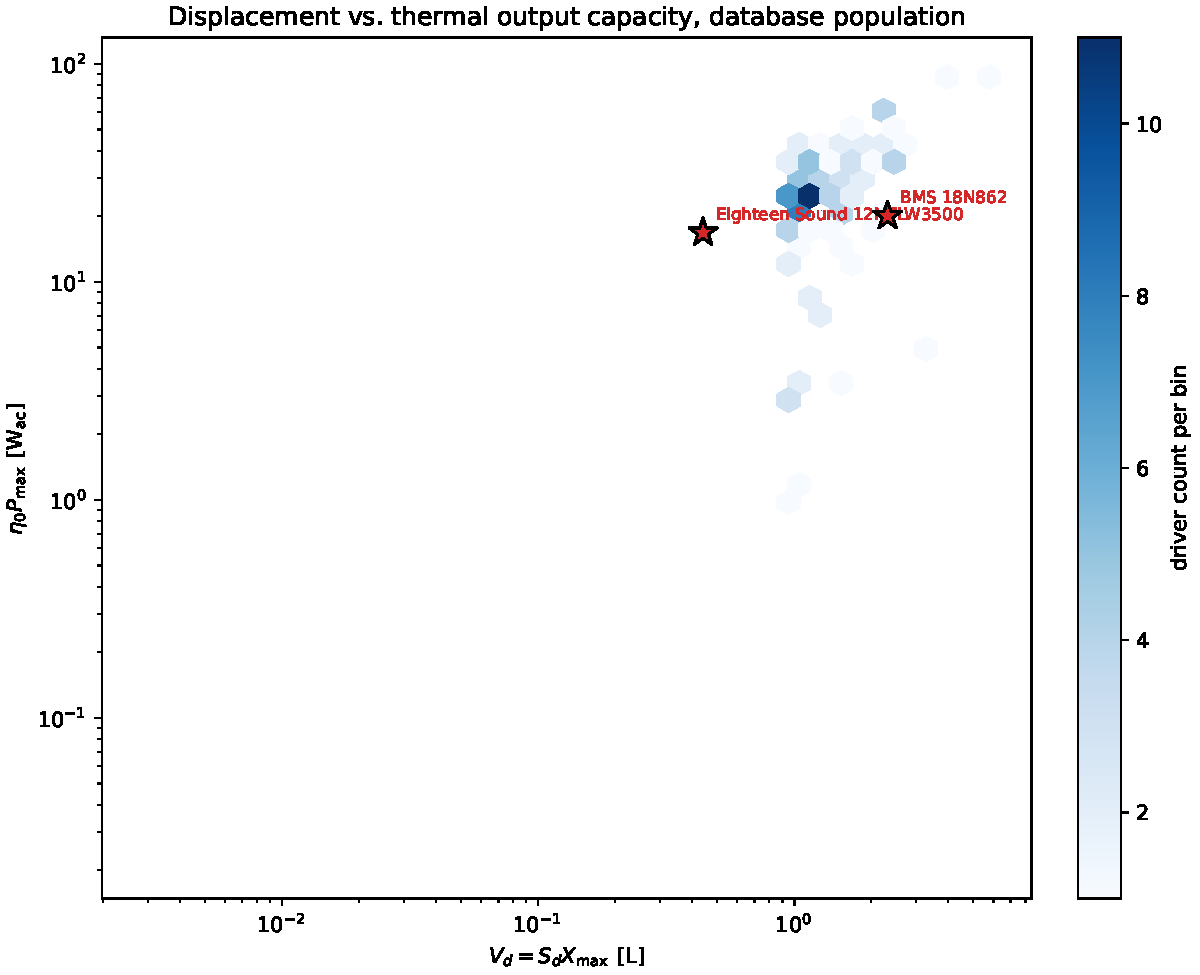
\includegraphics[width=\columnwidth]{../figures/fig_database_pareto}
	\caption{Frozen candidate population in the $(\Vd,\eta_0\Pmax)$ plane,
	shown as a binned density so that no individual record is disclosed. The
	two candidates selected in \cref{app:example} are marked. Aggregate
	population evidence only; the counts behind it are in
	\cref{tab:database-summary}.}
	\label{fig:database-pareto}
\end{figure}

\begin{table*}[htbp]
\centering
\caption{Private driver-database evidence summary at the worked unit counts (aggregate counts only. The accompanying manifest supplies the full source hash, parser, and filter definitions).}
\label{tab:database-summary}
\begin{tabular}{lr}
\toprule
quantity & value\\
\midrule
source hash (SHA-256, first 12 hex) & \texttt{0a5edbd1868e}\\
retained rows & 1342\\
skipped rows (missing required fields) & 537\\
sub-manifold role candidates (15--21in) & 246\\
sub-manifold role feasible (2 total) & 1\\
sub-manifold role Pareto front & 1\\
upper-bass role candidates (8--15in) & 592\\
upper-bass role feasible (1/channel) & 146\\
upper-bass role Pareto front & 41\\
both role tests feasible at worked counts (size-unrestricted) & 1\\
\bottomrule
\end{tabular}
\end{table*}


The observation this evidence supports is deliberately narrow: in this
frozen population, under this scenario, the candidates selected for the two
roles occupy different regions of the $(\Vd,\eta_0\Pmax)$ plane, differing
chiefly in displacement volume at comparable thermal output capacity.
Overlap between driver-level role populations does not establish that one
stereo full-band system meets both channel reference bases within the
allowed sizes and counts; that system question is evaluated next.

\subsection{Crossover and architecture sensitivity}
\label{sec:procedure-architecture}

The crossover is swept in \SI{5}{\hertz} increments before selecting the
worked system. For the public Dayton/Faital pair of
\cref{app:example}, \SI{60}{\hertz} fails upper-driver excursion and
Doppler gates, \SI{65}{\hertz} remains Doppler-limited, and
\SIrange{70}{80}{\hertz} is feasible. The upper role continues to gain
margin above \SI{80}{\hertz}, but those points are driver-only
counterfactuals because the illustrative manifold declares
\SI{80}{\hertz} as its highest nominal crossover. The implemented
low-pass must still suppress manifold output above its validated acoustic
band.

\begin{figure}[htbp]
	\centering
	\includegraphics[width=\columnwidth]{../figures/fig_split_sensitivity}
	\caption{Worked-pair crossover sensitivity. Hard-feasible points at or
	below the declared manifold ceiling are distinguished from rejected
	points and driver-only counterfactuals above the ceiling. The selected
	\SI{80}{\hertz} point maximizes upper-driver margin only within the
	declared feasible interval; it is not a universal optimum.}
	\label{fig:split-sensitivity}
\end{figure}

\begin{table*}[htbp]
\centering
\caption{Crossover sensitivity with every other scenario input fixed. Candidate entries are hard-feasible/preferred-margin record counts in the declared role pools. The public worked pair is re-aligned and its enclosure recalculated at every crossover. Points above the declared manifold ceiling are driver-only counterfactuals (CF), not valid manifold recommendations. $F/P$ denotes hard-feasible/preferred-margin records.}
\label{tab:split-sensitivity}
\scriptsize
\setlength{\tabcolsep}{2pt}
\begin{tabular}{rrrrrrrl}
\toprule
$f_{\mathrm{sp}}$ [Hz] & valid & sub $F/P$ & upper $F/P$ & worked $\xi_s/\xi_u$ & $V_{b,u}$ [L] & $d_{\mathrm D,u}$ & status\\
\midrule
60 & yes & 1/1 & 62/21 & 0.80/1.09 & 46.2 & 0.025 & reject\\
65 & yes & 1/1 & 89/44 & 0.80/0.91 & 33.0 & 0.021 & reject\\
70 & yes & 1/1 & 110/76 & 0.80/0.76 & 25.3 & 0.018 & preferred\\
75 & yes & 1/1 & 129/102 & 0.80/0.65 & 20.2 & 0.016 & preferred\\
80 & yes & 1/1 & 146/115 & 0.80/0.56 & 16.6 & 0.014 & preferred\\
85 & no & 1/1 & 171/134 & 0.80/0.50 & 15.7 & 0.012 & preferred; CF\\
90 & no & 1/1 & 183/146 & 0.80/0.46 & 15.7 & 0.011 & preferred; CF\\
95 & no & 1/1 & 199/165 & 0.80/0.43 & 15.7 & 0.010 & preferred; CF\\
100 & no & 1/1 & 216/176 & 0.80/0.40 & 15.7 & 0.009 & preferred; CF\\
105 & no & 1/1 & 234/191 & 0.80/0.38 & 15.7 & 0.008 & preferred; CF\\
110 & no & 1/1 & 244/204 & 0.80/0.36 & 15.7 & 0.007 & preferred; CF\\
115 & no & 1/1 & 250/219 & 0.80/0.34 & 15.7 & 0.007 & preferred; CF\\
120 & no & 1/1 & 257/228 & 0.80/0.32 & 15.7 & 0.006 & preferred; CF\\
\bottomrule
\end{tabular}
\end{table*}


To test whether the two-role result is merely assumed, a factorial study
compares it with the favourable full-band stereo baseline B5. The inputs
span room volumes of 40, 60 and \SI{90}{\cubic\meter}; nominal crossovers
of 60, 80, 100 and \SI{120}{\hertz}; upper edges of 200, 250 and
\SI{350}{\hertz}; and low-bass targets of 105, 110 and \SI{115}{dB}, with
the independent upper target \SI{5}{dB} lower. Packaging searches use
15--21-inch low-bass drivers in even totals of 2, 4 or 6;
8--15-inch upper drivers at one or two per channel; and 10--18-inch
full-band drivers at one or two per channel.

Because unreported voice-coil inductance makes a 200--\SI{350}{\hertz}
role unevaluable, the primary comparison requires reported $\Le$. In the
canonical 60-\si{\cubic\meter}, 80/250-\si{\hertz},
110/105-\si{dB} case, 119 unique low-bass records and 301 upper-bass
records are feasible at one or more allowed counts, whereas no full-band
record is feasible. The split architecture therefore occupies the
data-complete system Pareto frontier alone in that case. If missing
inductance is permitted, one full-band record survives, but its
upper-band validity remains unresolved; reducing the assumed stereo bass
summing credit from 6 to \SI{3}{dB} removes even that survivor.

\begin{figure}[htbp]
	\centering
	\includegraphics[width=\columnwidth]{../figures/fig_architecture_comparison}
	\caption{Outcome of the 108-scenario architecture study. Each scenario
	is evaluated with the same physical and electronics gates and then
	compared on six separate system objectives. Empty or single-architecture
	fronts are reported rather than converted into a success-shaped score.}
	\label{fig:architecture-comparison}
\end{figure}

\begin{table*}[htbp]
\centering
\caption{Architecture comparison over the declared domestic/mastering factorial. Each target has 36 cases: three room/longest-dimension pairs, four crossovers, and three upper-band edges. Upper-bass target is 5 dB below the listed low-bass target. Upper/full candidates must report $L_e$. ``Separate radiators'' compares the two-role architecture at every tested crossover; ``80-Hz manifold'' removes split designs above the declared manifold ceiling. Counts are scenario cases, not combinatorial driver-pair counts.}
\label{tab:architecture-comparison}
\scriptsize
\setlength{\tabcolsep}{3pt}
\begin{tabular}{lrrrrrrr}
\toprule
basis & $L_{\mathrm{sub}}$ [dB] & split feas. & full feas. & split only & mixed & full only & neither\\
\midrule
separate radiators & 105 & 36 & 24 & 12 & 24 & 0 & 0\\
80-Hz manifold & 105 & 18 & 24 & 6 & 12 & 12 & 6\\
separate radiators & 110 & 36 & 16 & 20 & 16 & 0 & 0\\
80-Hz manifold & 110 & 18 & 16 & 10 & 8 & 8 & 10\\
separate radiators & 115 & 36 & 0 & 36 & 0 & 0 & 0\\
80-Hz manifold & 115 & 18 & 0 & 18 & 0 & 0 & 18\\
\bottomrule
\end{tabular}
\end{table*}


Across all tested crossovers, split systems are feasible in all 36 cases at
each target. Full-band systems share the Pareto front in 24 of 36 cases at
\SI{105}{dB} and 16 of 36 at \SI{110}{dB}, but none at
\SI{115}{dB}. Enforcing the illustrative \SI{80}{\hertz} manifold ceiling
removes the split architecture from the 100- and
\SI{120}{\hertz} cases by definition; this creates full-band-only and
neither-feasible outcomes. The two panels therefore separate a
driver/system tradeoff from an external manifold-integration limit.

This supports role specialization for the stated population and envelope,
not a universal motor theorem. Different amplifier, package, room, target
or candidate inputs can restore a full-band frontier member, and the tool
is designed to report it when they do. Current regional price is considered
only after the technical shortlist; the canonical strict case has no
data-complete full-band finalist for a symmetric price comparison.

\subsection{Rank robustness}
\label{sec:procedure-robustness}

Public data is imprecise, and the lexicographic order is a policy. The
ranking is therefore recomputed under declared perturbations---$\Xmax$
scaled by $\pm25\%$, $\Pmax$ shifted by $\pm\SI{3}{dB}$, alternative room
leakage corners, and alternative reasonable lexicographic
orders---and the overlap of the top-$k$ shortlist with the baseline is
reported (\cref{fig:rank-robustness}). If fewer than $k$ baseline records
are feasible, retention is normalized by the records actually available,
not by $k$.

\begin{figure}[htbp]
	\centering
	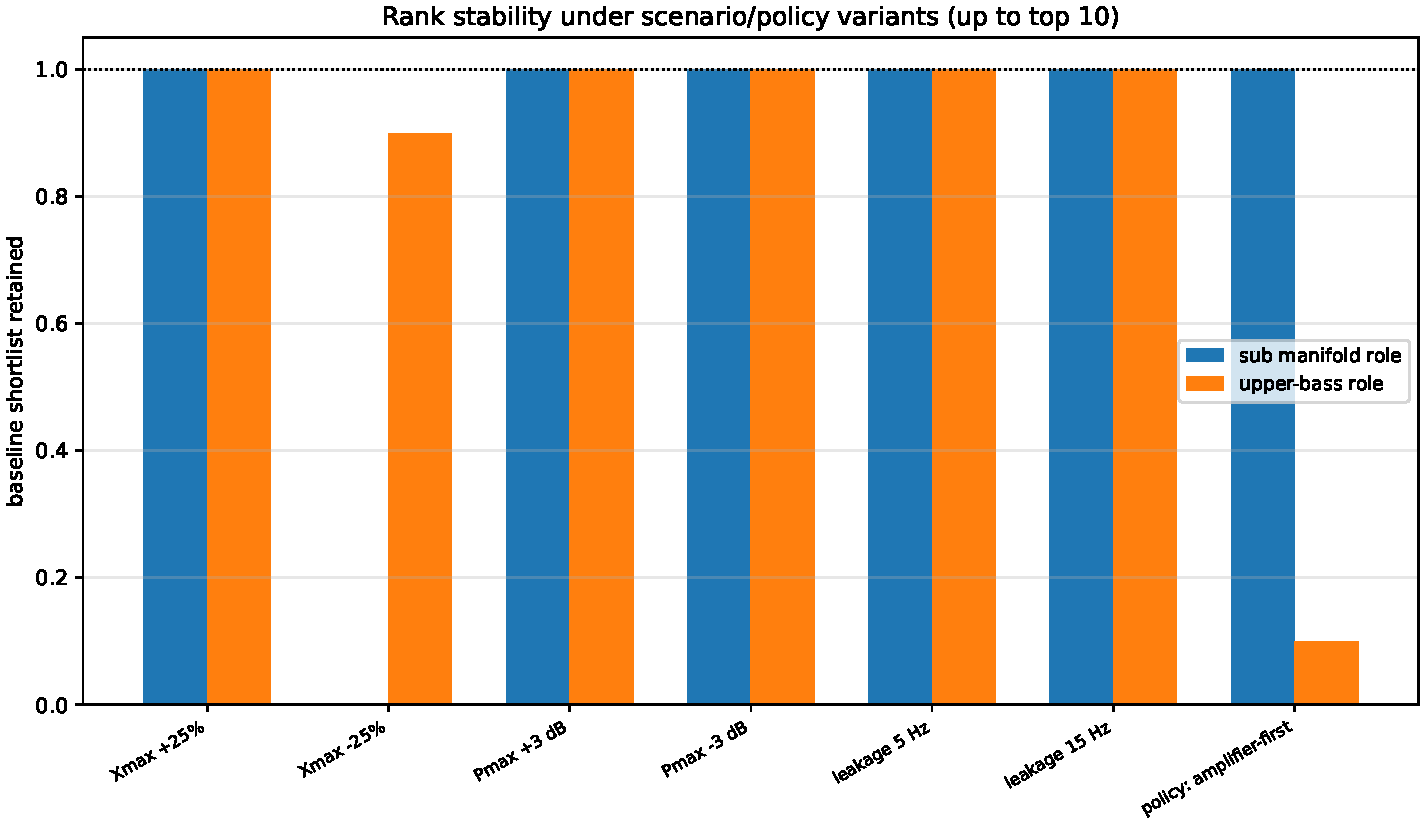
\includegraphics[width=\columnwidth]{../figures/fig_rank_robustness}
	\caption{Top-$k$ shortlist overlap with the baseline ranking under
	declared datasheet, room, and policy perturbations, for both roles. A
	high overlap indicates that the shortlist does not depend on the precise
	value of an uncertain input; a low one identifies where the
	recommendation is provisional.}
	\label{fig:rank-robustness}
\end{figure}

Power-rating and leakage variants retain every baseline record in both
roles. Reducing $\Xmax$ by 25\% removes the sole feasible two-driver
low-bass record and changes one member of the upper top ten. Reordering by
amplifier headroom retains the sole low-bass record but only one of the
upper ten. The low-bass result is therefore binary rather than evidence of
a broad stable shortlist; $\Xmax$ convention and upper-role policy remain
material and are reported with the recommendation.

This is a sensitivity analysis of the decision procedure. It is
\emph{not} physical validation: it does not test the nonlinear indicators
against measured large-signal behaviour. Such validation would require
public $Bl(x)$, $K_{\mathrm{ms}}(x)$, or distortion-headroom measurements
for a comparable subset of candidates, and is identified in
\cref{sec:conclusion} as the principal outstanding item.

\section{Conclusion}
\label{sec:conclusion}

The problem posed in \cref{sec:intro} was: given a room, one listening
position, and a target level, choose sealed bass driver(s) that reach it
with the least non-correctable distortion.

\textbf{Two regimes, two drivers.} A sealed driver's output near $F_s$ is
capped by displaced volume $\Vd=\Sd\Xmax$ (\cref{cor:onlyVd}); above $f_x$
\eqref{eq:fx} it is capped by dissipation $\eta_0\Pmax$ \eqref{eq:SPLT}. The
motor materials bound (\cref{thm:bound}) proves $EBP\cdot u^2\le
K_{\mathrm{mat}}\beta_{\max}$: stroke and corner rate trade off through the
same coil-mass fraction, so no single voice-coil motor maximizes both at
once. A sub role and an attack role are therefore best served by two
physically different drivers.

\textbf{Sealed, not vented.} \Cref{app:vented} shows a vented alignment's
low-frequency asymptote is $24$\,dB/oct, not sealed's $12$; that below
tuning its excursion is bounded only by drive, not by the box; and that
reaching a realistic in-room target drives port air velocity past the
empirical turbulence-onset threshold. A sealed box forfeits at most an
octave of extension for a given volume, recovered mostly for free from the
room.

\textbf{Room gain closes the low end.} Below $f_{\mathrm{pz}}=c/2L_{\max}$
the demand curve flattens, and a sealed corner placed at
$F_c\simeq f_{\mathrm{pz}}$ is flat in-room to the leakage corner with no
EQ. A vented box's steeper roll-off is not rescued the same way.

\textbf{The selection procedure is datasheet-only.} Every quantity in
\cref{sec:procedure} is computable from ten datasheet rows, with no free
parameter beyond the room, the target level, and the distortion budget.

\textbf{Verdict.} An optimal sealed bass monitor for one listening
position, in a room large enough to matter, is a two-driver system: a
high-$\Vd$, long-throw driver sealed and corner-tuned to the room's
pressure zone, plus a light, strongly motored driver above the split,
sharing a common baffle plane. No single driver saturates both invariants
at once, and no enclosure other than sealed lets the room pay for the last
octave without the costs quantified in \cref{app:vented}. This verdict
holds within the DSP-corrected, room-integrated premise of
\cref{sec:assumptions}; where amplifier headroom, rather than distortion
or room gain, is the binding constraint, \cref{app:vented} names a
legitimate narrower-purpose alternative.

\Cref{sec:prevwork}'s review is closed by these results: $EBP$ remains a
legitimate enclosure-\emph{type} screen but does not extend to an absolute
performance ranking --- the excursion regime's ranking is $\Vd$ alone, the
dissipation regime's is $\eta_0\Pmax$. The model is LTI to leading order in
$x/\Xmax$ and excludes directivity/breakup above $ka\approx1$; distortion
laws are order-of-magnitude ranking predictors, not $\pm1$\,dB THD
forecasts. A companion preprint \cite{audioshape-preprint} gives the
complete derivations, model-limitation list, and a worked numerical example
(reproduced here in \cref{app:example}), together with an open-source
reference implementation.


\section*{Acknowledgment, Data, and Code Availability}
The candidate population analysed in \cref{sec:procedure} is a locally held
export of the VituixCAD community driver database. That file is obtained
separately and is \emph{not} redistributed with this report: only its
source description, SHA-256 hash, parser metadata, filter definitions, and
aggregate counts and population plots are published, in
\path{papers/26325/data/driver_database_manifest.json}. The driver
records used in the worked example of \cref{app:example} are taken from the
manufacturers' public datasheets; the exact source URLs and SI inputs are
recorded in the manifest, and the computed results are summarized in
\cref{tab:worked-pair}. The reference implementation, the figure and table
generation script, the canonical scenario file, the unit tests, and the
companion explanatory preprint \cite{audioshape-preprint}, which carries the
full derivations omitted here, are available at
\url{https://github.com/luchp/audioshape}; the version used here is
identified in the archived release accompanying this report.
The author declares a competing interest: he develops loudspeaker
design software commercially at SenseMagic.

\appendix
\section{Worked example}
\label{app:example}

This appendix applies the complete procedure to the canonical scenario of
\cref{sec:scope-scenario}. Both drivers are named models, and every
parameter used is taken from a public manufacturer datasheet. The
accompanying data manifest records the exact source URLs and SI input
records; \cref{tab:worked-pair} summarizes the computed results and is the
authoritative source where a number below is rounded.

\subsection*{Selected system}

\textbf{Low-bass manifold.} Two Dayton Audio UMII18-22 units arranged as
one mechanically opposed pair, permitting first-order reaction-force
cancellation under matched drive and mounting. Driver mismatch and
mounting tolerances leave residual force. The suffix ``22'' denotes dual
\SI{2}{\ohm} voice coils; the manufacturer's one-way linear excursion is
\SI{28}{\milli\meter}. The two drivers carry one common mono signal and share the
manifold target of \SI{110}{dB} \emph{in total} at
$r_{\mathrm{listen}}=\SI{3}{\meter}$ (basis B3); each has its own amplifier
channel. The $4\Vas$ cap binds at \SI{993}{\liter} per driver, giving
$\Qtc\simeq0.592$ and $F_c\simeq\SI{24.6}{\hertz}$. The resulting
\SI{1.99}{\cubic\meter} total enclosure is retained as a visible packaging
cost rather than hidden by a role-wide cap.

\textbf{Upper bass.} One FaitalPRO 12HP1030 per independent stereo
channel in \SI{16.6}{\liter}, giving $\Qtc\simeq0.539$ and
$F_c\simeq\SI{80}{\hertz}$, exactly at the split. Each channel meets its
own \SI{105}{dB} target at \SI{3}{\meter} (basis B4) with no credit from
the opposite channel. Publication calculations use the current official
manufacturer record, including $\Sd=\SI{518}{\centi\meter\squared}$,
$\Vas=\SI{35.9}{\liter}$ and
$\Xmax=\SI{12.45}{\milli\meter}$.

\subsection*{Demand and gates}

With $V_{\mathrm{room}}=\SI{60}{\cubic\meter}$ and
$L_{\max}=\SI{6}{\meter}$, $f_{\mathrm{pz}}\simeq\SI{28.6}{\hertz}$. Under
the declared \SI{10}{\hertz} leakage corner the worst low-bass demand
occurs at the bottom of the band, \SI{15}{\hertz}, and equals
\SI{4.57}{\liter} of peak displaced volume for the manifold as a whole
(\cref{tab:room-sensitivity}), hence about \SI{2.29}{\liter} per driver.

The realized alignment differs from the preferred $\Qtc^\ast=0.55$ because
the box cap binds. Its finite-band correction is not assumed free: any
boost is charged to \cref{eq:Preq,eq:Ereq,eq:Ireq}, excursion and burst
response, and the resulting worst-case values are checked against the
gates.
Across the complete \SIrange{15}{80}{\hertz} band the low-bass units run at
approximately $\xi_x\simeq0.689$ steady and
$\xi_x^{\mathrm{tr}}\simeq0.795$ for the declared one-cycle burst family.
The largest amplifier-budget utilization is about 0.642, inside the
\SI{90}{\volt}, \SI{15}{\ampere}, \SI{500}{\watt} continuous and
\SI{1}{\kilo\watt} burst limits and the driver's own rating.

The upper-bass channel uses $\xi_x\simeq0.485$ steady and
$\xi_x^{\mathrm{tr}}\simeq0.557$; its Doppler first-sideband ratio is
0.0138 and its largest amplifier-budget utilization is about 0.597.
Both roles are inside the hard $\Xmax$ boundary and the 0.80 preferred
excursion margin.
\Cref{fig:worked-system}
collects the separately reported indicators for both roles, and
\cref{fig:output-electrical} shows the corresponding output margin and
electrical utilization across each role's band.

\begin{figure}[htbp]
	\centering
	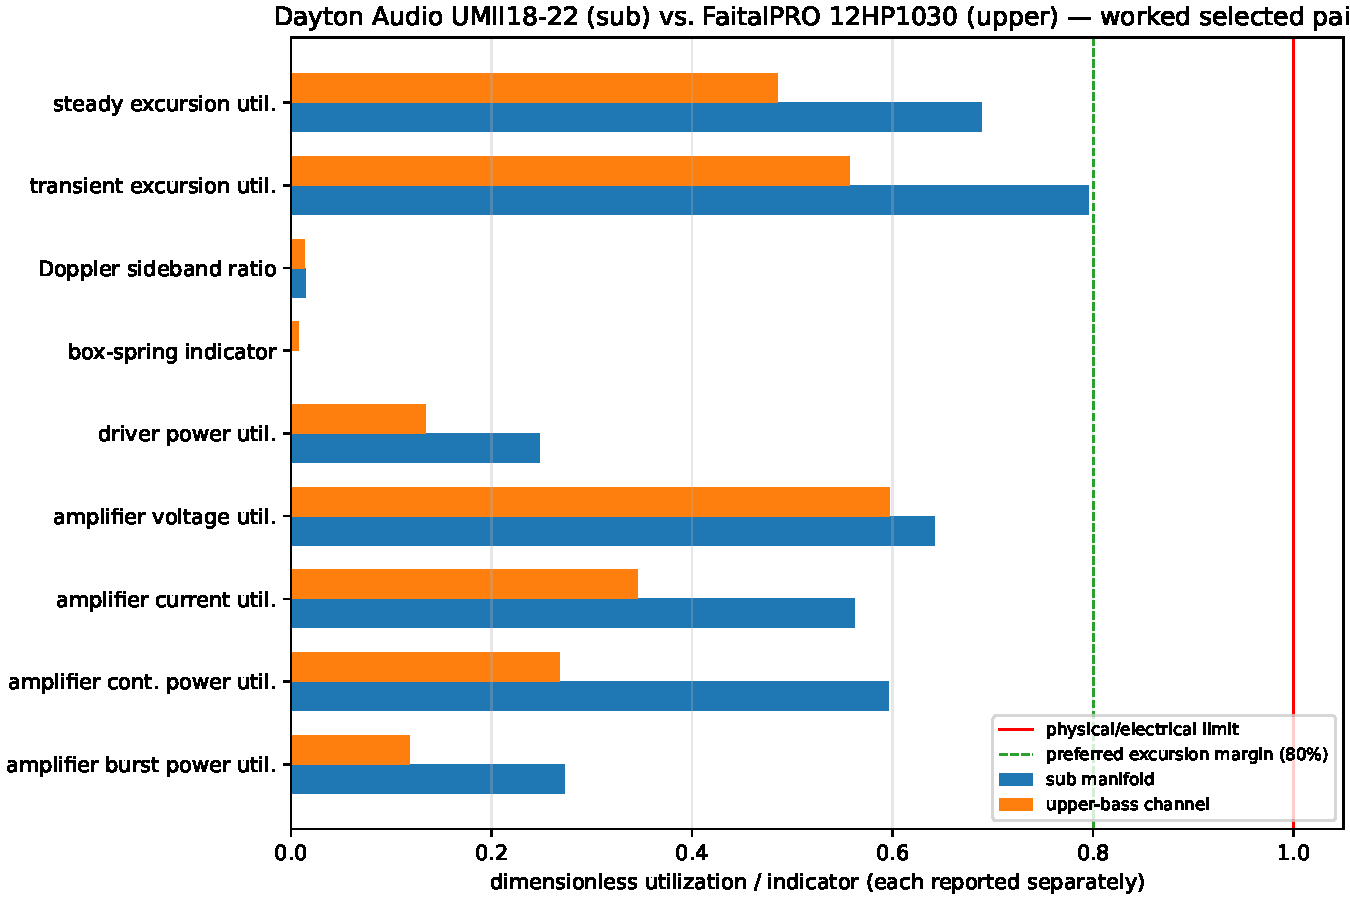
\includegraphics[width=\columnwidth]{../figures/fig_worked_system}
	\caption{Complete worked system: the dimensionless indicators of
	\cref{eq:riskvec} for the mono low-bass manifold and for one independent
	stereo upper-bass channel, against the hard limit and the preferred
	excursion margin. Each indicator is reported separately; none is summed
	with another.}
	\label{fig:worked-system}
\end{figure}

\begin{table*}[htbp]
\centering
\caption{Worked selected pair: Dayton Audio UMII18-22 (mono sub manifold, 2 identical units in an even, symmetrically opposed pairing -- permitting first-order reaction-force cancellation under matched drive and mounting; the even count is a hard mechanical-layout constraint, not a ranking-policy preference -- each with its own amplifier channel, aggregate target 110 dB for the manifold, not per driver) and FaitalPRO 12HP1030 (upper-bass, one unit per independent stereo channel, target 105 dB per channel). Pareto front number is one-based and is against this report's frozen private-database candidate pool for each role.}
\label{tab:worked-pair}
\small
\begin{tabular}{p{4.0cm}p{5.1cm}p{5.1cm}}
\toprule
 & Dayton UMII18-22 (sub) & FaitalPRO 12HP1030 (upper)\\
\midrule
public source & Dayton Audio official UMII18-22 specification sheet & FaitalPRO official 12HP1030 product data (8 ohm)\\
role, units & mono sub manifold, 2x (even, opposed pairs for first-order force cancellation when matched), aggregate target 110 dB for the manifold & stereo upper-bass, 1x per channel, target 105 dB per channel\\
$V_d$ per driver [L] & 3.32 & 0.64\\
$\eta_0 P_{\max}$ [W$_{\mathrm{ac}}$] & 4.63 & 10.32\\
$F_s$ / $Q_{ts}$ & 22 Hz / 0.530 & 45 Hz / 0.303\\
$f_L=\Re/2\pi\Le$ [Hz] & 581 & 589\\
box per driver: $V_b$, $F_c$ & 993 L, 24.6 Hz & 16.6 L, 80.0 Hz\\
$Q_{tc}$ & 0.592 & 0.539\\
worst steady excursion util. & 0.69 & 0.48\\
worst transient excursion util. & 0.80 & 0.56\\
worst voltage [V rms @ Hz] & 56.9 @ 28.6 & 53.7 @ 80.0\\
worst current [A rms @ Hz] & 8.4 @ 80.0 & 5.2 @ 250.0\\
worst power [W @ Hz] & 298 @ 80.0 & 134 @ 250.0\\
Pareto front / status & 1 / feasible & 1 / feasible\\
\bottomrule
\end{tabular}
\end{table*}


\subsection*{Reading the result}

Three points matter more than the specific models.

First, the binding trade differs by role. For the low-bass manifold the
$4\Vas$ cap fixes a very large enclosure and its correction demand; for the
upper-bass channel the crossover controls excursion and Doppler margin.
Neither is visible from an output-ceiling comparison alone.

Second, the two roles are served by candidates from different regions of
the descriptor plane (\cref{fig:database-pareto}). Within this candidate
population and scenario, the alternatives that rank close to each selection
do so for role-specific reasons---greater $\Vd$ at higher electrical demand
for the low-bass role, greater $\eta_0\Pmax$ at lower $f_L$ for the
upper-bass role---and their Pareto and policy statuses are reported in
\cref{tab:worked-pair} rather than reduced to a single score.

The earlier hard-$\Qtc$/role-volume formulation selected a costly
high-flux professional 18-inch driver largely because it excluded
high-$\Qts$, high-stroke alternatives geometrically. Under the revised
policy the UMII18-22 pays explicitly for its box and equalization, yet
remains Pareto-optimal. The selected model is therefore a consequence of
the declared physical and electronics tradeoffs, not of treating
$F_s< f_{\mathrm{pz}}$ or $\Qtc\le0.55$ as mandatory.

Third, the result is conditional on the room. \Cref{tab:room-sensitivity}
shows how the required displaced volume, and hence the driver count, moves
with the assumed leakage corner; a less favourable corner is absorbed here
by the manifold's excursion margin, but that margin is finite and is
reported rather than assumed.

\section{Why sealed loading was chosen here}
\label{app:vented}

Sealed loading is an architectural choice for this application, not the
outcome of a general topology contest. This appendix states the reasoning
and its limits.

A vented alignment is a fourth-order system \cite{small1973vented}: the box
compliance and the port's acoustic mass and resistance add a degree of
freedom to the sealed operator \cref{eq:ode}, to which it reduces exactly
as the port mass and resistance grow without bound. Compared with a sealed
box of the same volume, it buys roughly an octave of extension and higher
passband sensitivity---a decisive advantage when amplifier power, not
displacement or room gain, is the binding constraint.

Four properties make it the less convenient choice for the architecture of
\cref{sec:intro-arch}.

\textbf{Below-tuning excursion.} Below the tuning frequency the enclosure
supplies little restoring force, so cone excursion is limited by the drive
signal rather than by the alignment. Standard practice adds a protective
high-pass filter below tuning, which is entirely workable, but it removes
output in exactly the region where the pressure-zone branch of
\cref{eq:Vdem} would otherwise be exploited. The sealed alternative bounds
displacement at every frequency down to DC without an additional protective
element, which makes the excursion gates of \cref{sec:risk-policy}
sufficient on their own.

\textbf{Steeper low-frequency slope.} The vented low-frequency asymptote is
steeper than the sealed $12$\,dB/oct, so the approximate complementarity
with the room's pressure-zone branch \cref{eq:Fsrule} does not carry over
directly, and correction toward the bottom of the band starts from a larger
deficit.

\textbf{Port behaviour.} Near tuning most of the output passes through the
port, and the port air velocity at a given target scales as
$v_{\mathrm{port}}\approx2\pi r_{\mathrm{listen}}p_t/
(\rho_0\omega_b S_{\mathrm{port}})$. At the levels and frequencies of this
scenario a small port would run well above the velocity at which
compression, turbulence noise, and nonlinear behaviour become significant
\cite{salvatti2002,vanderkooy1998}. This is a design constraint on port
geometry, not a defect of vented loading: large flared ports, several
ports, or a passive radiator address it, at the cost of enclosure volume,
baffle area, or an additional moving part. A passive radiator removes the
port mechanism entirely while retaining the fourth-order alignment and the
below-tuning excursion behaviour.

\textbf{System integration.} The manifold of \cref{sec:intro-arch} already
uses several active drivers for displacement and first-order
reaction-force cancellation under matched opposed-pair operation, each
with its own amplifier channel. In that context the extra tuning element,
the protective filter, and the port geometry constraint add system
complexity without addressing the binding constraint, which
\cref{app:example} shows is enclosure volume and excursion rather than
amplifier power.

None of this establishes that sealed loading is generally superior. Under a
different constraint set---limited amplifier power, limited enclosure
volume with a higher extension requirement, or a room without usable
pressure-zone gain---a vented or passive-radiator alignment is the
better-matched choice, and the gates of \cref{sec:risk-policy} would have
to be re-derived for its fourth-order model.


\bibliography{../refs}
\bibliographystyle{jaes}

% Suppress the class's black missing-photo placeholder in the review draft.
% Add \biography with an actual photo for the final publication package.
\makeatletter
\authorgdtrue
\makeatother

\end{document}
